%!TEX program = xelatex
\documentclass[cn,hazy,blue,11pt,normal]{elegantnote}
\title{人工智能 - PRP 笔记}

\author{林楠}
\institute{Shanghai Jiao Tong University}

\date{\zhtoday}

\usepackage{array}
\usepackage{tikz}
\usepackage{pgfplots}
\usepackage{float}

\begin{document}

\maketitle

\newpage
\tableofcontents
\newpage

\section{神经网络基础知识}

\subsection{MP神经元}


一个神经元会同时接受多个信号,然后将这些信号乘以一定权重求和,再用函数处理再输出新的信号。对神经元的输入进行处理,以获得输出的函数称为激活函数。
\begin{figure}[htpb] %h:当前位置, t:顶部, b:底部, p:浮动页
    \centering
    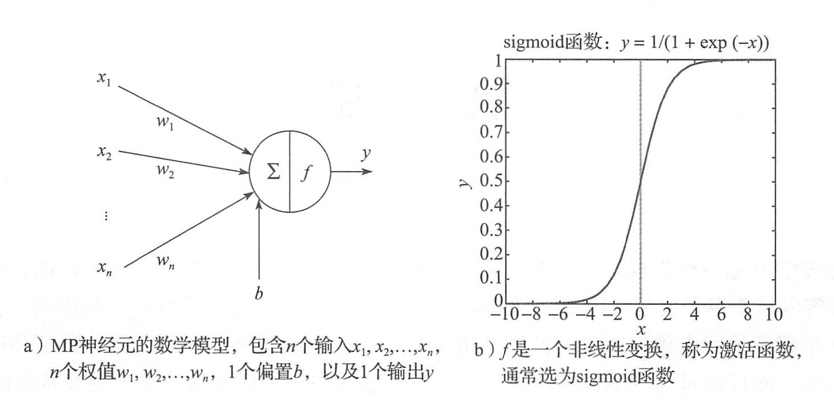
\includegraphics[width=0.8\textwidth]{./fig/MP神经元.png}
    \caption{MP神经元}
    \label{fig:MP神经元}
\end{figure}

定义:

\begin{enumerate}
    \item 外部因素 $\langle x_1,x_2,\ldots,x_n \rangle =x$
    \item 权重 $(w_1,w_2,\ldots,w_n) = w$
    \item $w\cdot x = \sum_j w_jx_j$
    \item $b=-\text{threshold}$
    \item 激活函数 $\sigma$
\end{enumerate}

运作过程:
\begin{enumerate}
    \item 确定输入和输出
    \item 找到一种或多种算法,可以从输入得到输出
    \item 找到一组已知答案的数据集,用来训练模型,估算$w$和$b$
    \item 一旦新的数据产生,输入模型,就可以得到结果,同时对$w$和$b$进行校正
\end{enumerate}

计算函数:
\[
z = wx+b, \text{and then calculate } a = \sigma(z)
\]

输入 $(x_1,x_2,\ldots,x_n)$ 对应的权重分别是 $(w_1,w_2,\ldots,w_n)$,阀值为 threshold,我们有:
\[
    \text{output} = \begin{cases}
        0, \text{if } \sum_jw_jx_j \le \text{threshold} \\
        1, \text{if } \sum_jw_jx_j \ge \text{threshold}
    \end{cases}
\]

\subsection{神经网络}

\begin{figure}[H] %h:当前位置, t:顶部, b:底部, p:浮动页
    \centering
    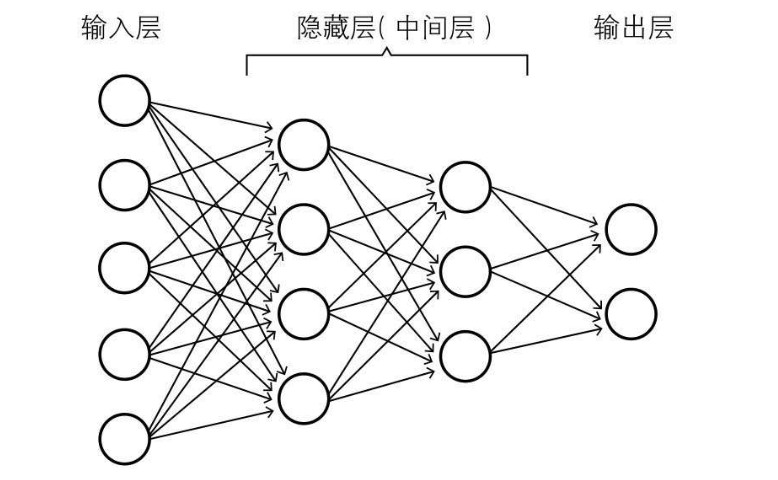
\includegraphics[width=0.8\textwidth]{./fig/输入层、隐藏层、输出层.png}
    \caption{输入层、隐藏层、输出层}
    \label{fig:输入层-隐藏层-输出层}
\end{figure}

定义:
\begin{enumerate}
    \item $a^{[0]}= X = (x_1,x_2,x_3,\ldots,x_n)$
    \item 层数指的是隐藏层的层数,输入层不算在其中(或是第0层)
    \item
        \[
            a_i^{[l]}: i\text{ is the node index in the layer}, l\text{ is the layer index}
        \]
\end{enumerate}

\begin{figure}[H] %h:当前位置, t:顶部, b:底部, p:浮动页
    \centering
    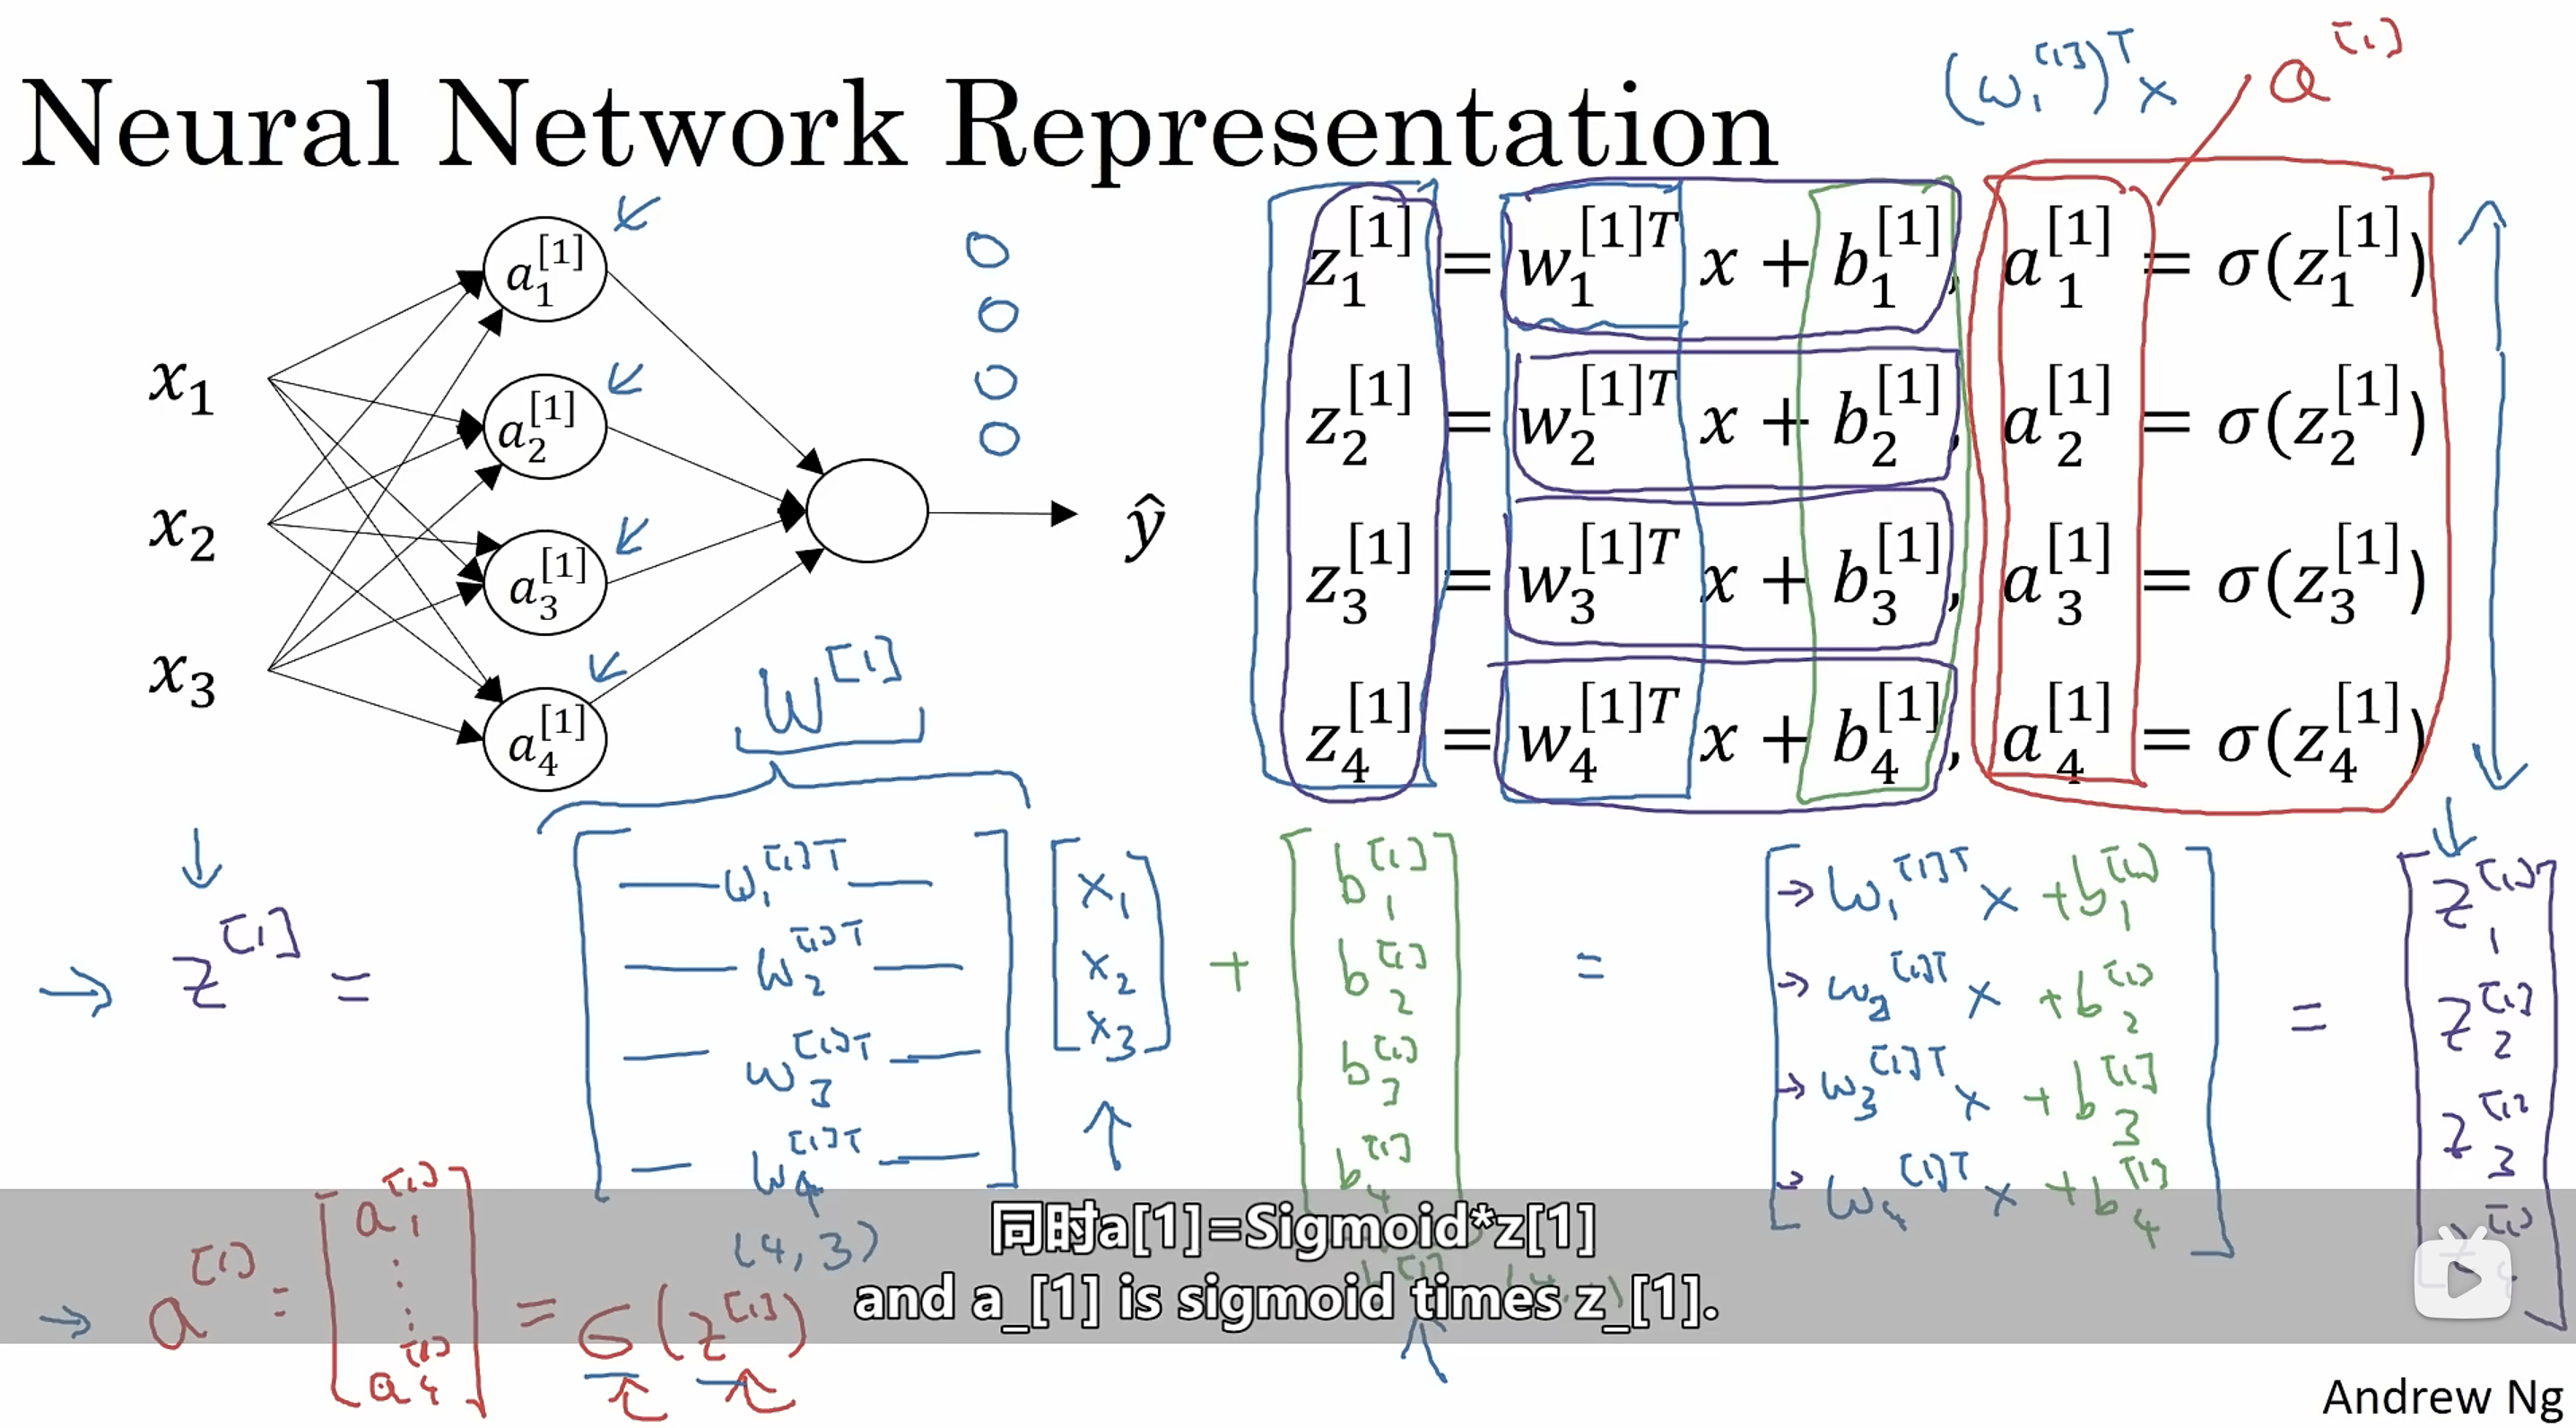
\includegraphics[width=\textwidth]{./fig/浅层神经网络计算.png}
    \caption{浅层神经网络计算}
    \label{fig:浅层神经网络计算}
\end{figure}

Given input $x=a^{[0]}$, 这里我们有四个节点三个输入,$W=w^{T}$, 纬度是$(4,3)$, 且 $a^{[0]}$ 纬度是 $(3,1)$

\[
    z^{[1]} = W^{[1]}a^{[0]}+b^{[1]}, \text{and then } a^{[1]}=\sigma(z^{[1]})
\]

我们这样标记第 $i$ 个数据:
\[
	a^{[1](i)} = \sigma(z^{[1](i)}) = \sigma(w^{[1]}a^{[0](i)}+b^{[1]})
\]

\subsection{激活函数}
\begin{figure}[H] %h:当前位置, t:顶部, b:底部, p:浮动页
    \centering
    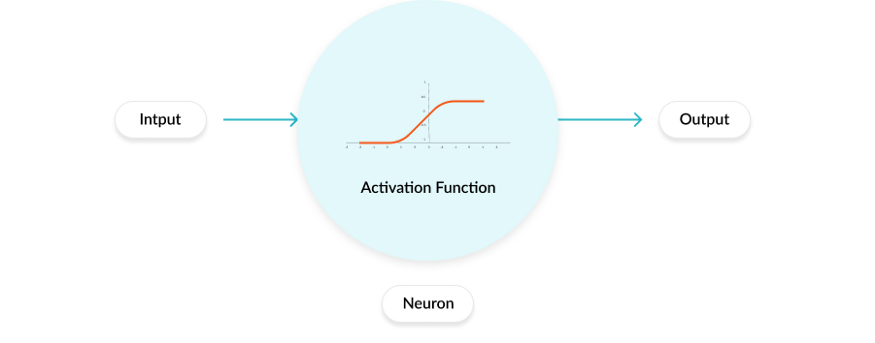
\includegraphics[width=0.8\textwidth]{./fig/激活函数.png}
    \caption{激活函数}
    \label{fig:激活函数}
\end{figure}
\begin{enumerate}
    \item 非线性 sigmoid 函数
        \[
            \text{sigmoid}(x) = \frac{1}{1+e^{-x}}
        \]
        \begin{figure}[H]
            \centering
            \begin{tikzpicture}
                \begin{axis}[
                    xmin= -5, xmax= 5,
                    ymin= 0, ymax = 1,
                    axis lines = middle,
                ]
                \addplot[domain=-5:5, samples=100]{1/(1+e^(-\x))};
                \end{axis}
            \end{tikzpicture}
            \caption{sigmoid函数}
            \label{sigmoid函数}
        \end{figure}
    \item 双曲正切 tanh 函数
        \[
            \tanh (x) = \frac{e^{x}- e^{-x}}{e^{x}+e^{-x}}
        \]
        \begin{figure}[H]
            \centering
            \begin{tikzpicture}
                \begin{axis}[
                    xmin= -5, xmax= 5,
                    ymin= -1, ymax = 1,
                    axis lines = middle,
                ]
                    \addplot[domain=-5:5, samples=100]{tanh(\x)};
                \end{axis}
            \end{tikzpicture}
            \caption{tanh函数}
            \label{tanh函数}
        \end{figure}
    \item 校正线性单元 ReLU 函数
        \[
        \text{ReLU}(x) = \max(0,x)
        \]
        \begin{figure}[H]
            \centering
            \begin{tikzpicture}
                \begin{axis}[
                    xmin= -5, xmax= 5,
                    ymin= -5, ymax = 5,
                    axis lines = middle,
                ]
                    \addplot[domain=-5:0, samples=100]{0};
                    \addplot[domain=0:5,samples=100]{\x};
                \end{axis}
            \end{tikzpicture}
            \caption{ReLU函数}
            \label{ReLU函数}
        \end{figure} 
    \item 渗漏校正线性单元 LReLU 和参数校正线性单元 PReLU 函数
        \[
        \text{LReLU(x)} = \text{PReLU(x)} = \begin{cases}
            1, x\ge 0 \\ ax, x<0
        \end{cases}
        \]
        
        LReLU 中 $a\in (0,1)$ 是个固定值,而 PReLU 中  $a\le 1$ 是个通过学习得到的参数。

        \begin{figure}[H]
            \centering
            \begin{tikzpicture}
                \begin{axis}[
                    xmin= -5, xmax= 5,
                    ymin= -5, ymax = 5,
                    axis lines = middle,
                ]
                    \addplot[domain=0:5, samples=100]{1};
                    \addplot[domain=-5:0, samples=100]{0.4*\x};
                \end{axis}
            \end{tikzpicture}
            \caption{LReLU和PReLU函数}
            \label{LReLU和PReLU函数}
        \end{figure}
    \item 指数线性单元 ELU 函数
        \[
        \text{ELU}(x) = \begin{cases}
            1,x\ge 0\\a(e^{x}-1),x<0
        \end{cases}
        \]
        $a\ge 0$ 是一个可调参数。
        \begin{figure}[H]
            \centering
            \begin{tikzpicture}
                \begin{axis}[
                    xmin= -5, xmax= 5,
                    ymin= -5, ymax = 5,
                    axis lines = middle,
                ]
                    \addplot[domain=0:5, samples=100]{1};

                    \addplot[domain=-5:0, samples=100]{0.4*(e^\x-1)};
                \end{axis}
            \end{tikzpicture}
            \caption{ELU函数}
            \label{ELU函数}
        \end{figure}

    \item 软加函数 softplus 函数
        \[
        f(x) = \ln(1+e^{x})
        \]
        \begin{figure}[H]
            \centering
            \begin{tikzpicture}
                \begin{axis}[
                    xmin= -5, xmax= 5,
                    ymin= -5, ymax = 5,
                    axis lines = middle,
                ]
                    \addplot[domain=-5:5, samples=100]{ln(1+e^\x)};
                \end{axis}
            \end{tikzpicture}
            \caption{softplus函数}
            \label{softplus函数}
        \end{figure}
        
\end{enumerate}



\end{document}

